\documentclass[border=4pt,convert={density=800,size=500x300,outext=.png}]{standalone}
\usepackage{tikz}
\usetikzlibrary{automata,positioning}
\begin{document}
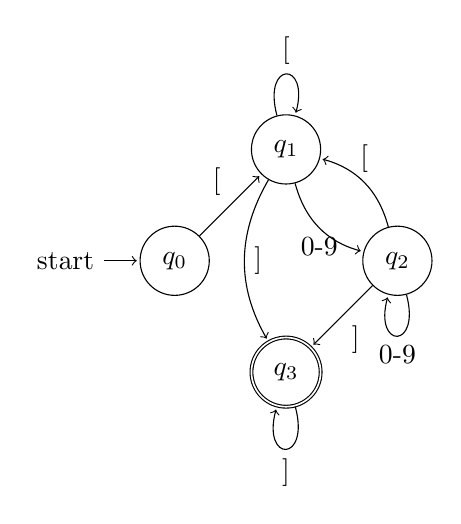
\begin{tikzpicture}[shorten >=1pt,node distance=2cm,on grid,auto] 
   \node[state,initial] (q_0)   {$q_0$}; 
   \node[state] (q_1) [above right=of q_0] {$q_1$}; 
   \node[state] (q_2) [below right=of q_1] {$q_2$}; 
   \node[state, accepting] (q_3) [below right=of q_0] {$q_3$}; 
    \path[->] 
    (q_0) edge  node {[} (q_1)
    (q_1) edge [bend right] node [below] {0-9} (q_2)
          edge [loop above] node {[} ()
    (q_2) edge  node {]} (q_3)
          edge [loop below] node {0-9} ()
    (q_2) edge [bend right] node [above] {[} (q_1)
    (q_1) edge [bend right] node {]} (q_3)
    (q_3) edge [loop below] node {]} ();
\end{tikzpicture}
\end{document}  
